\chapter{Ensuring group consistency in Pithos}
\label{chp:GROUP_INCONSISTENCY}

This appendix described, in chronological order, the steps taken to ensure group consistency. It provides initial findings, discusses the reasons for inconsistency and introduces the proposed solutions.

\section{Initial approach}
The initial approach to achieve group consistency was to have every peer inform all other peers when it was moving from one group to another. If a peer is removed from the network due to churn, another peer has to discover that the peer has left, which is done with timeouts. If a request times out, the peer making the request informs the group of the peer that left.

\begin{figure}[htbp]
 \centering
 \includegraphics[clip=true, viewport=0mm 0mm 460mm 212mm, width=\columnwidth]{gc_first}
 \caption{Group consistency before any improvements}
 \label{fig_gc_first}
\end{figure}
%
Figure \ref{fig_gc_first} shows an enlarged view of the perceived group size of every node in the group for the initial group consistency scheme. The lines running across the graph is due to nodes leaving the network and joining again at a later time.

From approximately 2925 s, a new peer joins the group and reports the group size as eight, when all other peers report the group size as seven. Multiple variations of these inconsistencies occurred during testing. A primary source of inconsistencies was the fact that it takes time to inform all group peers of a peer that left and that it takes time to inform all group peers of a peer that joined.

Issues also occurred because of how newly stored objects are handled. When a new peer joins the group, it starts to generate objects. The group super peer sends a joining peer a list of group peers. After this occurs, the group peers are informed of the new peer. A peer joining a group can immediately start to store objects at the request of other peers. This can happen before some peers are aware of the joining peer. The unaware peers will then get a message saying that an object has been stored on the new peer, before they are aware of the new peer. The solution was to assume that an object was generated by a valid peer and to add any unknown peer information contained in an object add message to the peers list in the group ledger.

Group inconsistency can arise because there might be some latent object add messages still enroute to peers, after the peer has already left the network and informed other peers of its leaving. This means that a peer has already left, but after it informed the group peers of its leaving and all group peers have removed the peer from memory, the group peers receive a message for an object that is supposedly now stored on the peer that just left. The mechanism mentioned above is initiated and the, now unknown, peer is again added to the peer list.

Many transient group states that led to inconsistencies were solved by the super peer storing the information of the last peer that left and the last peer that joined. Every time a new peer joins, the super peer informs the joining peer of the last peer that left. This allows the joining peer to ignore any latent object add messages received from the leaving peer. Any messages received from the last peer that left are ignored. This prevents latent messages from peers that left to affect the group view of peers.

\section{Peer starvation problem}
\begin{figure}[htbp]
 \centering
 \includegraphics[clip=true, viewport=0mm 0mm 455mm 212mm, width=\columnwidth]{gc_middle}
 \caption{Group consistency with starvation}
 \label{fig_gc_middle}
\end{figure}
%
The mentioned improvements created the issue shown in Figure \ref{fig_gc_middle}, where a peer will believe that another peer has left. The group will be informed of the peer that supposedly left, but is actually still present in the group. Because all peers will now ignore messages from the peer that supposedly left, including the super peer, all requests sent by the peer that supposedly left will be ignored. The requests will then timeout on the ignored peer and the ignored peer will remove all group peers. This isolates the peer and prevents any requests from being serviced.

The starvation was caused by peers not responding to requests. A scenario could occur where a peer did not contain a requested object or where the network bandwidth was limited, which prevented a response from arriving at a peer before the request timeout expired. In either of these two situation, the peer making the request was under the impression that the target peer had left the network. It then informed all other peers of this.

The solution to this issue was to adjust the timeout as a function of the available network bandwidth and to make sure every node always responded to a request, whether as a success or failure. Functionality was also added to the super peer to check whether a peer that was reported as having left, actually did leave the network.

Other issues were caused when group migration was enabled. A node might leave a group to move to another, but as the node leaves some peer that has not been informed of the peer leaving would make a request form the leaving peer. The leaving peer would respond to that request, which would have the requesting peer add the peer back into the group. This could cause the situation where peers existed in multiple groups.

The solution to this was to include the group membership information in every request message. A peer's membership can be uniquely identified by the IP address and port of the group's super peer. If a peer receives a message with a different group address than its own, it ensures that that peer is not part of its group.

This also solved the case where Peer A requested an object from Peer B, just as Peer B was leaving the group. Peer B will already be in its new group when receiving the request from Peer A. Peer B will see that the request originated from outside its group, so will not add the new peer to its group. If it contains the requested object, it will however still respond with the object. When Peer A receives the object, it will detect that it was sent from another group and remove Peer B from its group ledger. In this way, the request was successfully handled and group consistency is maintained.

\section{Final solution}
\begin{figure}[htbp]
 \centering
 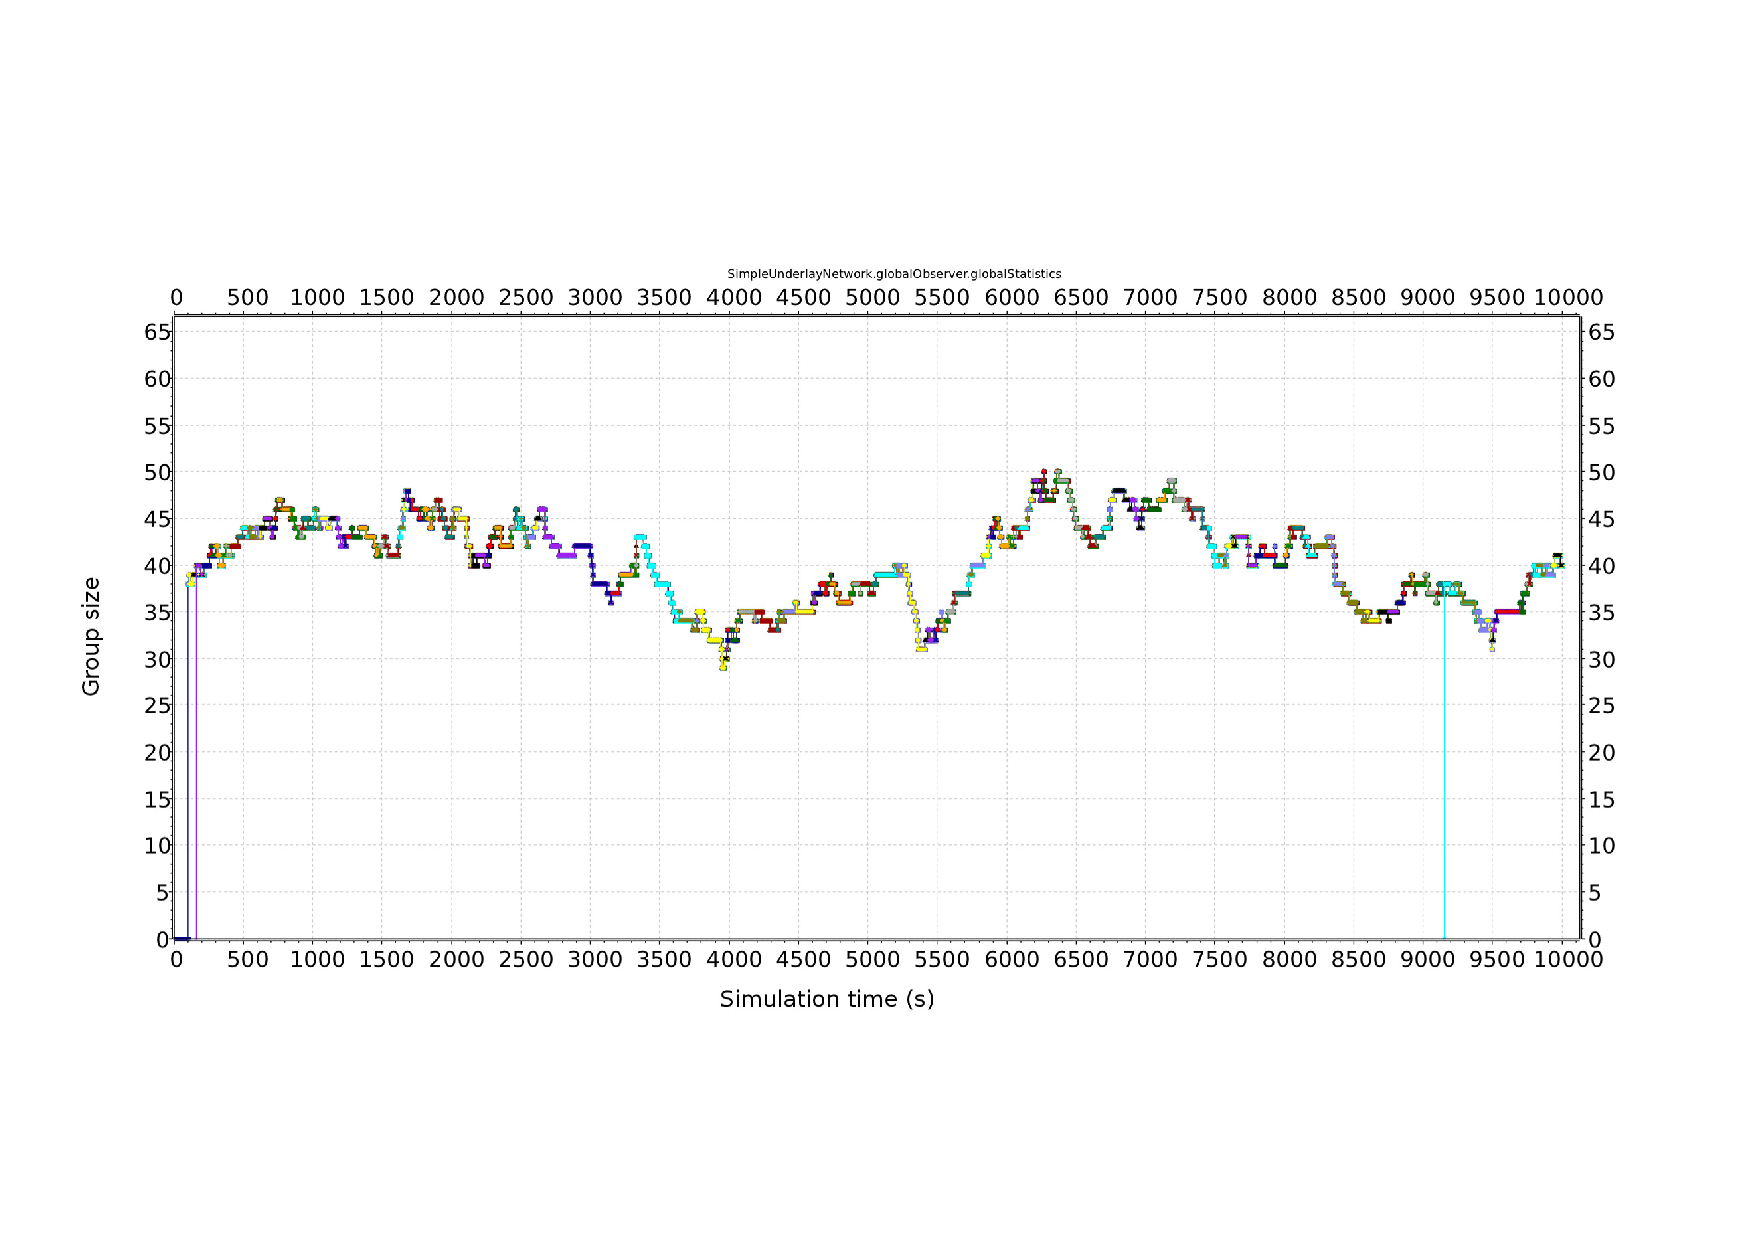
\includegraphics[clip=true, viewport=12mm 35mm 275mm 165mm, width=\columnwidth]{gc_final_png}
 \caption{Group consistency after all improvements}
 \label{fig_gc_final_app}
\end{figure}
%
Figure \ref{fig_gc_final_app} shows the group consistency after all improvements were added for a larger group than the previous two. Even with the larger group, complete consistency is achieved.

When object lifetime was tested, all requests were stopped after a certain period of time to speed up the simulation. This created an issue where group peers did not become aware of peers leaving the group, because no peers sent requests that could timeout. This prompted the addition of keep-alive messages.

Regular keep alive messages are sent to peers. If a peer does not respond to the message, that peer is removed from the group. The time between keep alive messages can be adjusted as a function of network churn. In order to reduce the load on the super peer, each peer randomly chooses a target peer and sends a keep-alive message, as explained in Section \ref{leave_design}.
